% Options for packages loaded elsewhere
\PassOptionsToPackage{unicode}{hyperref}
\PassOptionsToPackage{hyphens}{url}
%
\documentclass[
]{book}
\usepackage{amsmath,amssymb}
\usepackage{iftex}
\ifPDFTeX
  \usepackage[T1]{fontenc}
  \usepackage[utf8]{inputenc}
  \usepackage{textcomp} % provide euro and other symbols
\else % if luatex or xetex
  \usepackage{unicode-math} % this also loads fontspec
  \defaultfontfeatures{Scale=MatchLowercase}
  \defaultfontfeatures[\rmfamily]{Ligatures=TeX,Scale=1}
\fi
\usepackage{lmodern}
\ifPDFTeX\else
  % xetex/luatex font selection
\fi
% Use upquote if available, for straight quotes in verbatim environments
\IfFileExists{upquote.sty}{\usepackage{upquote}}{}
\IfFileExists{microtype.sty}{% use microtype if available
  \usepackage[]{microtype}
  \UseMicrotypeSet[protrusion]{basicmath} % disable protrusion for tt fonts
}{}
\makeatletter
\@ifundefined{KOMAClassName}{% if non-KOMA class
  \IfFileExists{parskip.sty}{%
    \usepackage{parskip}
  }{% else
    \setlength{\parindent}{0pt}
    \setlength{\parskip}{6pt plus 2pt minus 1pt}}
}{% if KOMA class
  \KOMAoptions{parskip=half}}
\makeatother
\usepackage{xcolor}
\usepackage{longtable,booktabs,array}
\usepackage{calc} % for calculating minipage widths
% Correct order of tables after \paragraph or \subparagraph
\usepackage{etoolbox}
\makeatletter
\patchcmd\longtable{\par}{\if@noskipsec\mbox{}\fi\par}{}{}
\makeatother
% Allow footnotes in longtable head/foot
\IfFileExists{footnotehyper.sty}{\usepackage{footnotehyper}}{\usepackage{footnote}}
\makesavenoteenv{longtable}
\usepackage{graphicx}
\makeatletter
\def\maxwidth{\ifdim\Gin@nat@width>\linewidth\linewidth\else\Gin@nat@width\fi}
\def\maxheight{\ifdim\Gin@nat@height>\textheight\textheight\else\Gin@nat@height\fi}
\makeatother
% Scale images if necessary, so that they will not overflow the page
% margins by default, and it is still possible to overwrite the defaults
% using explicit options in \includegraphics[width, height, ...]{}
\setkeys{Gin}{width=\maxwidth,height=\maxheight,keepaspectratio}
% Set default figure placement to htbp
\makeatletter
\def\fps@figure{htbp}
\makeatother
\setlength{\emergencystretch}{3em} % prevent overfull lines
\providecommand{\tightlist}{%
  \setlength{\itemsep}{0pt}\setlength{\parskip}{0pt}}
\setcounter{secnumdepth}{5}
\usepackage{booktabs}
\ifLuaTeX
  \usepackage{selnolig}  % disable illegal ligatures
\fi
\usepackage[]{natbib}
\bibliographystyle{plainnat}
\IfFileExists{bookmark.sty}{\usepackage{bookmark}}{\usepackage{hyperref}}
\IfFileExists{xurl.sty}{\usepackage{xurl}}{} % add URL line breaks if available
\urlstyle{same}
\hypersetup{
  pdftitle={FlowMax-Q Manual},
  pdfauthor={Srirama Bhamidipati},
  hidelinks,
  pdfcreator={LaTeX via pandoc}}

\title{FlowMax-Q Manual}
\author{Srirama Bhamidipati}
\date{Last Updated 2024-02-23 15:50:50.244832 Europe/Amsterdam}

\begin{document}
\maketitle

{
\setcounter{tocdepth}{1}
\tableofcontents
}
\hypertarget{preface}{%
\chapter{Preface}\label{preface}}

This manual is divided into two parts. The first part deals with Creating and Editing Networks in QGIS environment while the second part deals with Using the QGIS plugin.

\hypertarget{part-buidling-network-in-qgis}{%
\part{Buidling network in QGIS}\label{part-buidling-network-in-qgis}}

\hypertarget{introduction}{%
\chapter{Introduction}\label{introduction}}

\begin{itemize}
\tightlist
\item
  Economy based scenarios are to be modified in the trade-databases.
\item
  Resilience based scenarios (GIS) fall into 2 categories: node-based, edge-based. These in turn fall into 2 categories: editing geometries; editing attributes
\item
  Technology based scenarios will affect the demand (freight composition)
\item
  Policy based scenarios will affect the route and mode choices (freight composition)
\end{itemize}

\hypertarget{scenarios}{%
\chapter{Scenarios}\label{scenarios}}

The image below shows the underlying structure of constructing scenarios

\begin{figure}
\centering
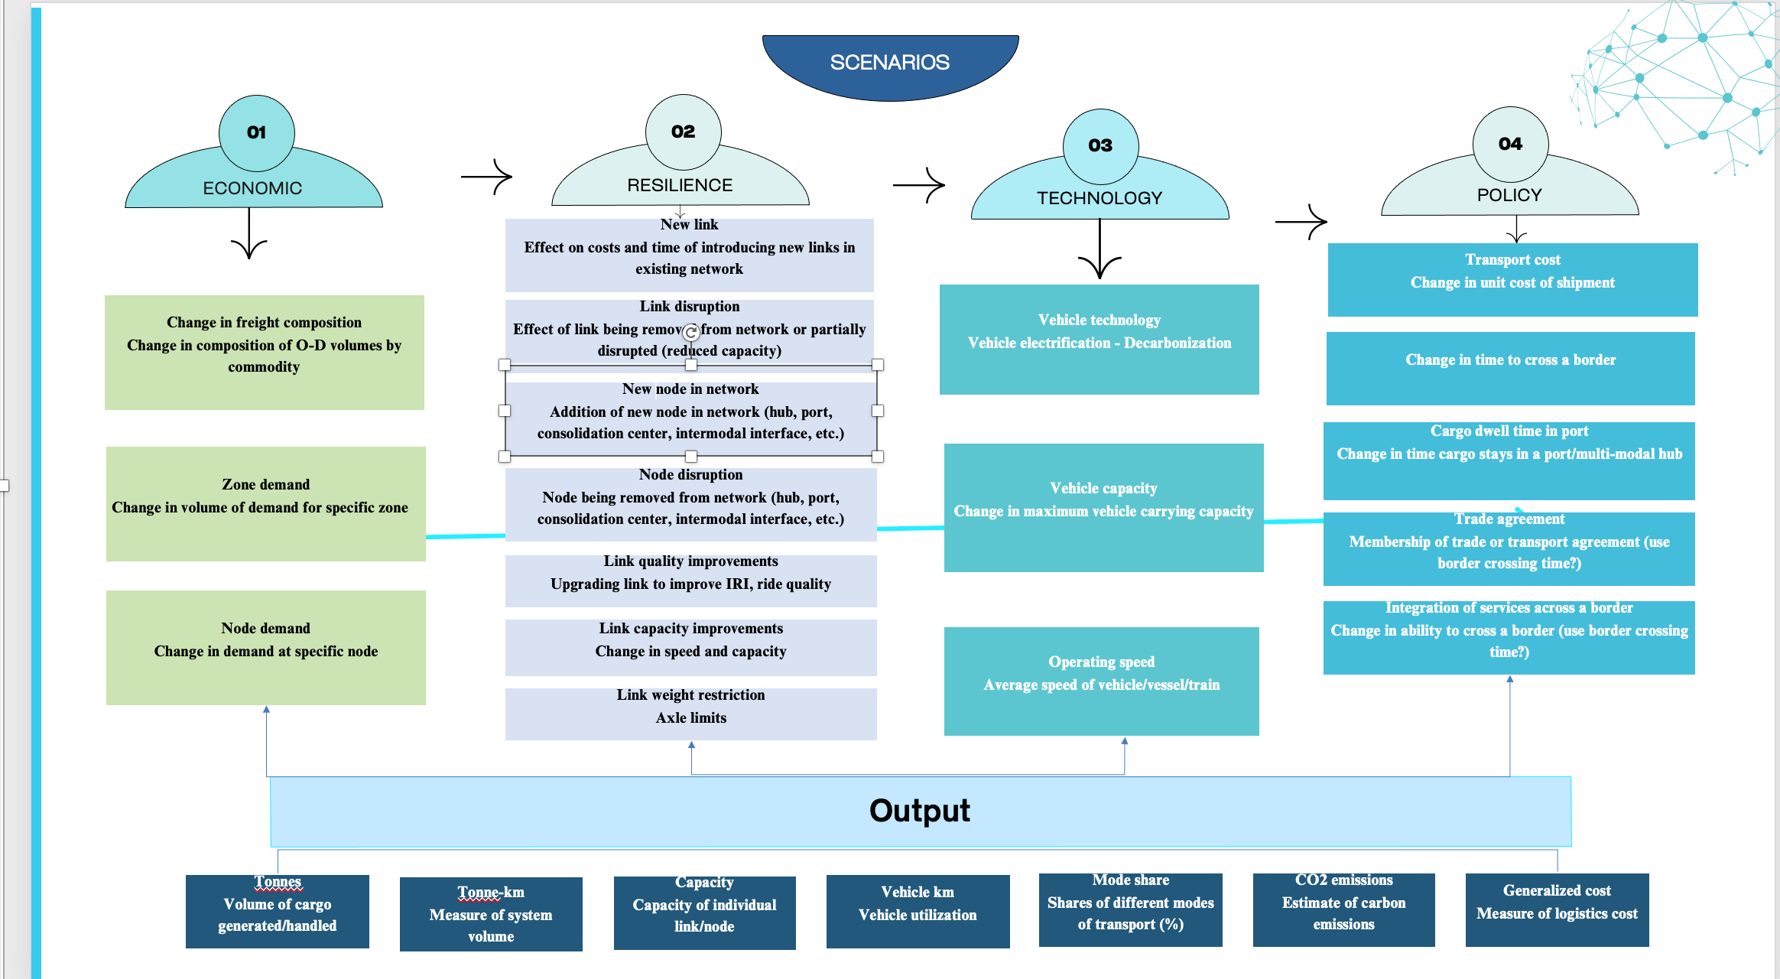
\includegraphics{"./Picture1.png"}
\caption{Scenarios}
\end{figure}

\hypertarget{adding-links}{%
\chapter{Adding Links}\label{adding-links}}

Is the new link connecting to an existing link but not at an existing node location?

\begin{itemize}
\tightlist
\item
  Yes ? First assure that there is a node each for the source and destination of this new link
  - Yes ? create a line between source and destination nodes.
  - No? First create a node
\item
  No? Is the new link connecting to an existing node location?
  - Yes? First assure that there is a node at the new location at the end of the new link (if the link starts from existing node)
\end{itemize}

\hypertarget{removing-links}{%
\chapter{Removing Links}\label{removing-links}}

\hypertarget{removing-a-link-disabling-links}{%
\section{Removing a Link (disabling links)}\label{removing-a-link-disabling-links}}

It is advised not to remove a link (line-geometry) in GIS.
It is recommended that you use the `active' attribute in the link shapefile:
- edit this attribute to a value 0 (integer) instead of 1(integer) for the link in consideration.\\
- Assigning a 0 will remove the `active = 0' link(s) from path building of the Flowmax algorithm

\hypertarget{adding-back-an-existing-disabled-link}{%
\section{Adding back an Existing (disabled) Link}\label{adding-back-an-existing-disabled-link}}

If you have set the `active' attribute to 0 to exclude the link(s) from analysis, you can always set the `active' attribute back to 1 to include the link(s) back into your analysis.

\hypertarget{modifying-node-attributes}{%
\chapter{Modifying Node Attributes}\label{modifying-node-attributes}}

Node file: All nodes come with predefined attributes. Whenever a new node is added, all the attributes should be assigned a value (either a known value or a default value)

To edit: right click the node file \textgreater{} open attribute table \textgreater{} start edit mode. Select any cell and change values as required. After editing, save the edits and close the table.

This applies to all scenarios where attribute values must be changed: capacity, speed, travel time, quality of links etc.

\hypertarget{modifying-edge-attributes}{%
\chapter{Modifying Edge Attributes}\label{modifying-edge-attributes}}

Link file: All links come with predefined attributes. Whenever a new link is added, all the attributes should be assigned a value (either a known value or a default value)

To edit: right click the link file \textgreater{} open attribute table \textgreater{} start edit mode. Select any cell and change values as required. After editing, save the edits and close the table.
This applies to all scenarios where attribute values must be changed: capacity, speed, travel time, quality of links etc.

\hypertarget{part-qgis-plugin}{%
\part{QGIS Plugin}\label{part-qgis-plugin}}

\end{document}
